In this section, we present a method for extracting behavioural~\emph{scenarios} from
system control programs and synthesising them into application-specific
integrated circuits implementing execution of these scenarios. We exploit the
existing formalism of Conditional Partial Order Graphs (CPOGs)~\cite{cpogs} for
synthesising scenarios. CPOGs are included~\cite{scenco} as a plugin in the WORKCRAFT
framework~\cite{workcraft}, which implements the scenario specification and
synthesis methods and handles the mapping of CPOGs into interconnection of
logic gates to produce a physical implementation of the system microcontroller.

\subsection{Extracting scenarios from programs}

We defined a \textit{scenario} to be a list of
operations that are executed in a specified order. Formally, a scenario
$s=(\mathcal{O},\prec)$ is a \textit{partial order}~(PO)~\cite{PO},
i.e. a binary precedence relation $\prec$ describing dependencies between a
set of operations $\mathcal{O}$ that satisfies two properties:

\begin{itemize}
    \item Irreflexivity: $\forall a \in \mathcal{O}, \neg(a \prec a)$
    \vspace{+1mm}
    \item Transitivity: $\forall a, b, c \in \mathcal{O}, (a \prec b) \wedge (b
    \prec c) \Rightarrow (a \prec c)$
\end{itemize}

To mine scenarios from blocks of instructions, we partially reuse the methodology
used for construction of the concurrency oracles from the previous section.

The methodology is realised as the following informal algorithm:

\begin{enumerate}
    \item Calculating the static data dependencies of the program.
    \item Construct the~\emph{unfolded} static dependencies
        graph~\footnote{Similar to one in the figure~\ref{fig-example-graph},
        but with with data-vertexes duplicated on every update.}
    \item Remove the data-vertexes preserving the transitive connections between
        instruction-vertexes.
    \item A~\emph{transitive closure} of the resulting graph will display the
        partial order on the set of events represented as instruction-vertexes.
\end{enumerate}

As an example, consider a program for the control unit of a hypothetical dual-motor
autonomous vehicle. The motor's velocity may be adjusted with the command~\hs{AdjustVelocity}
supplying the value in a register and referring the motor index (0 or 1). The status
of the system may be checked with the~\hs{SystemStatus} command, referring both motors
and a register to store the resulting status code.

\begin{figure}
\vspace{-10mm}
\centering
  \begin{minipage}[b]{0.5\textwidth}
\begin{minted}[linenos]{haskell}
Load R0 254
AdjustVelocity R0 0
AdjustVelocity R0 1
SystemStatus R2 0 1
\end{minted}
\vspace{5mm}
\end{minipage}
% \hfill
\begin{minipage}[b]{0.4\textwidth}
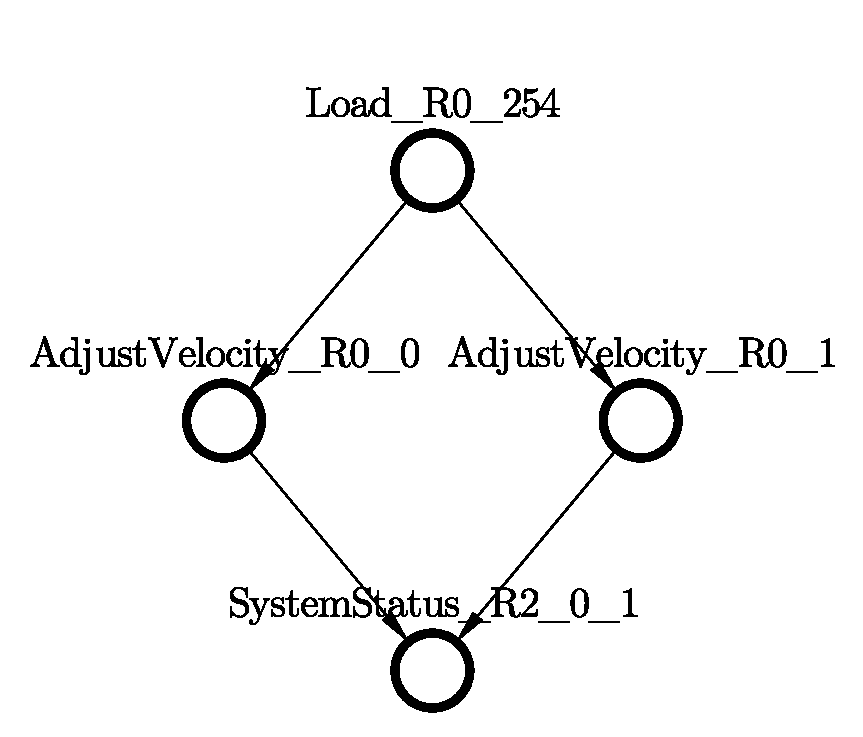
\includegraphics[scale=0.35]{img/ataed-scenario-1.pdf}
\end{minipage}
\caption{Simple behaviour scenario and the corresponding partial order.}
\end{figure}

Extraction of scenarios from programs enables us to use the associated methods for
compiling programs into application-specific hardware. The Conditional Partial
Order Graphs formalism enables synthesis of scenarios, allowing to compile them into
a circuit with some functionality shared.

Consider the above mentioned scenario synthesised with another one into a single
partial order which shares similar functionality.

\begin{figure}
\vspace{-4mm}
\centerline{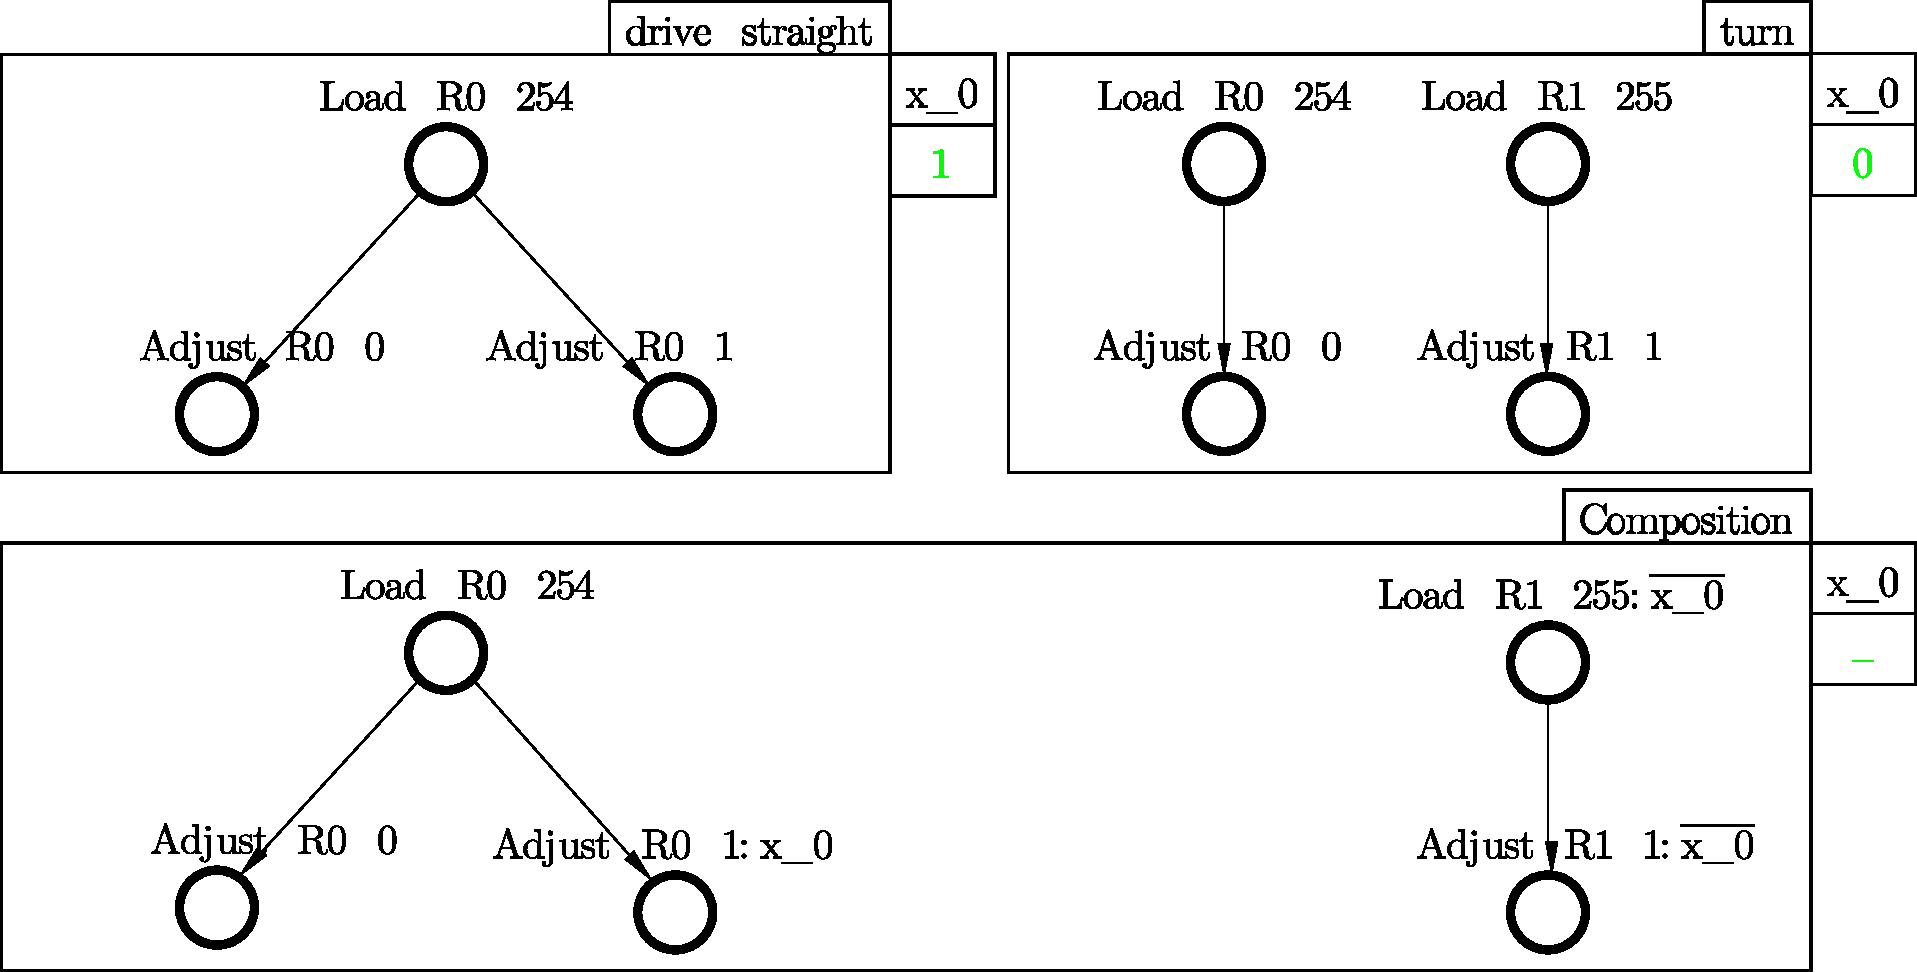
\includegraphics[scale=0.4]{img/ataed-composition.pdf}}
\caption{Two operation scenarios and their composition.\label{fig-scenarios}}
\vspace{-9mm}
\end{figure}

asdasdasdasdasdasd